% Created 2021-09-02 Thu 09:03
% Intended LaTeX compiler: pdflatex
\documentclass[presentation]{beamer}
\usepackage[utf8]{inputenc}
\usepackage[T1]{fontenc}
\usepackage{graphicx}
\usepackage{grffile}
\usepackage{longtable}
\usepackage{wrapfig}
\usepackage{rotating}
\usepackage[normalem]{ulem}
\usepackage{amsmath}
\usepackage{textcomp}
\usepackage{amssymb}
\usepackage{capt-of}
\usepackage{hyperref}
\usepackage{awesomebox}
\usepackage{booktabs}
\usepackage{placeins}
\usepackage{siunitx}
\usepackage{minted}
\usetheme[progressbar=frametitle,block=fill]{metropolis}
\usepackage{cleveref}
\usetheme{default}
\author{\emph{Tejaswin Parthasarathy}, Mattia Gazzola}
\date{\today}
\title{Introduction}
\subtitle{ME447: Comp. Design \& Dyn. of Soft Syst}
\hypersetup{
 pdfauthor={\emph{Tejaswin Parthasarathy}, Mattia Gazzola},
 pdftitle={Introduction},
 pdfkeywords={},
 pdfsubject={},
 pdfcreator={Emacs 28.0.50 (Org mode 9.3.6)},
 pdflang={English}}
\begin{document}

\maketitle

\begin{frame}[label={sec:org07bc4b3}]{Logistics}
\begin{itemize}
\item Office hours
\item Installation instructions up on Compass (Setup -> 00\_setup\_basics.pdf)
\item Will keep updating the hands-on lecture notes per module
\end{itemize}
\end{frame}
\section{Tentative plan}
\label{sec:orgd365964}
\begin{frame}[label={sec:orgcee45fd}]{Last class}
\begin{columns}
\begin{column}{0.5\columnwidth}
\begin{figure}[htbp]
\centering
\includegraphics[width=1\textwidth]{images/inverse_design.pdf}
\caption{Inverse design cycle}
\end{figure}
\end{column}

\begin{column}[c]{0.4\columnwidth}
\begin{itemize}
\item \alert{Compute}: How?
\item Analysis: How?
\end{itemize}
\end{column}
\end{columns}
\end{frame}

\begin{frame}[label={sec:org92788aa},fragile]{Content}
 \begin{itemize}
\item Motivate the need for/utility of \texttt{Python} + \texttt{shell} in comp. modeling
\item Introduction to \texttt{shell} (*nix) commands
\item \texttt{Python}: Setup/Installation
\item \texttt{Ipython shell} + \texttt{Jupyter} notebooks
\item Programming in \texttt{Python}: Basics to intermediate
\end{itemize}
\end{frame}

\begin{frame}[label={sec:org81c9e0d},fragile]{Quick survey}
 \begin{itemize}
\item \texttt{Python}?
\item Scientific computing in \texttt{Python} / other languages (if so, what)?
\item Use simulation for research/otherwise?
\item Familiarity with \texttt{terminal}?
\end{itemize}
\end{frame}
\section{Why python?}
\label{sec:orgf7f7f94}
\begin{frame}[label={sec:orga8eeb5b}]{Python is popular \footnote{Slide credits: \href{https://github.com/williamgrimes/teach\_python\_in\_notebooks/blob/master/python\_course.pdf}{William Grimes @ Github}}}
\begin{columns}
\begin{column}{0.35\columnwidth}
\begin{itemize}
\item Most visited tag on Stack Overflow among high-income nations
\item Used in
\begin{itemize}
\item Finance
\item Sciences
\item Webops
\item Business
\item \ldots{}
\end{itemize}
\end{itemize}
\end{column}
\begin{column}{0.65\columnwidth}
\footnotesize
\begin{figure}[htbp]
\centering
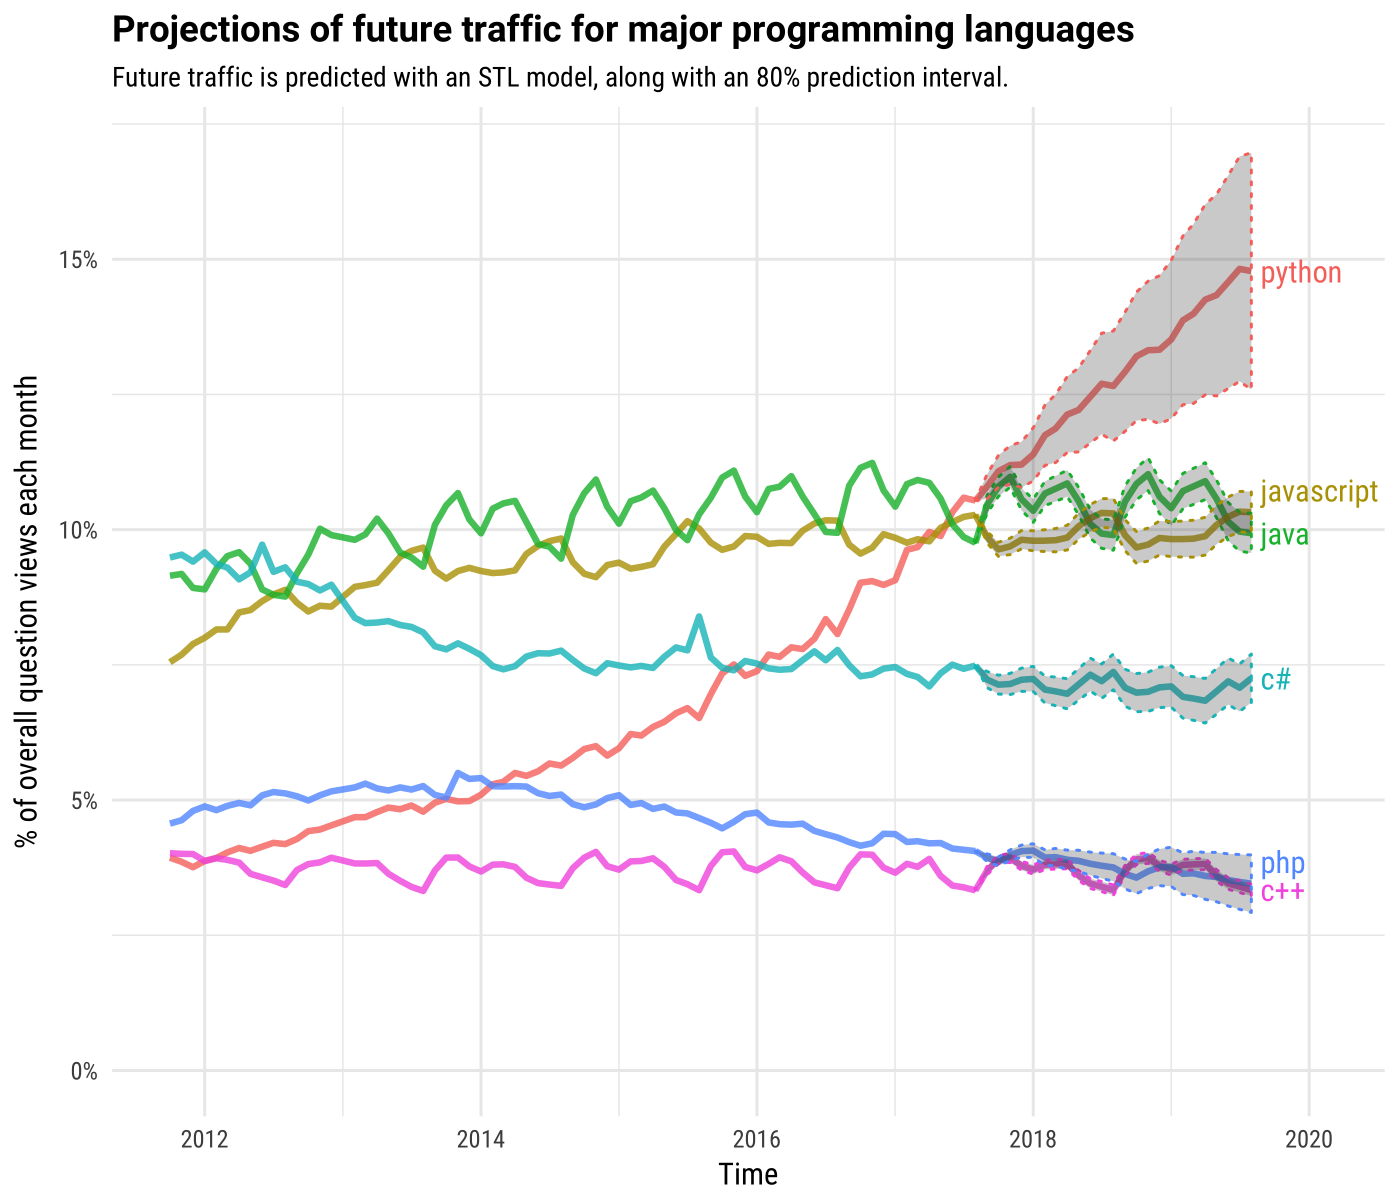
\includegraphics[width=1.0\textwidth]{images/so-projections.png}
\caption{Predictions}
\end{figure}
\end{column}
\end{columns}
\end{frame}

\begin{frame}[label={sec:org1e7f747}]{Python as a language}
\begin{itemize}
\item Free and open-source
\item Object oriented with sensible data structures
\item Interactive\footnote{\href{https://techfossguru.com/python-machine-learning-and-deep-learning/}{Techfossguru}} (and thus extensible)
\item Open source packages\footnote{\href{https://pypi.org/}{PyPi}} (323,575 as of August 25, 2021)
\item Widely used as an application/library API\footnote{\href{https://www.pluralsight.com/blog/software-development/why-python}{Pluralsight}}
\item \(\therefore\) productivity
\end{itemize}
\end{frame}

\begin{frame}[label={sec:org32efc53},fragile]{Interactive\footnote{\href{https://wiki.python.org/moin/IntegratingPythonWithOtherLanguages}{Wiki Python}}}
 \begin{itemize}
\item As a wrapper for other languages!
\begin{itemize}
\item \texttt{C++} : \texttt{Cython, SWIG, pybind ...}
\item \texttt{Fortran} : \texttt{F2Py, PyFort ...}
\item \texttt{Java} : \texttt{Jython, Javabridge ...}
\item \texttt{Perl} : \texttt{PyPerl, PyPerlish ...}
\item \texttt{...}
\end{itemize}
\item Enables game/web development, machine learning,
HPC \ldots{}
\end{itemize}
\end{frame}

\begin{frame}[label={sec:org923f9fa}]{FlappyBird      \footnote{\href{https://yanpanlau.github.io/2016/07/10/FlappyBird-Keras.html}{ FlappyBird-Keras}, \href{https://github.com/yanpanlau/Keras-FlappyBird/blob/master/qlearn.py}{Code} , \href{https://www.pygame.org/wiki/about}{Pygame}, \href{https://scikit-image.org/}{Scikit-image}, \href{https://www.tensorflow.org/}{TensorFlow}}}
\begin{columns}
\begin{column}[c]{0.35\columnwidth}
\footnotesize
\begin{figure}[htbp]
\centering
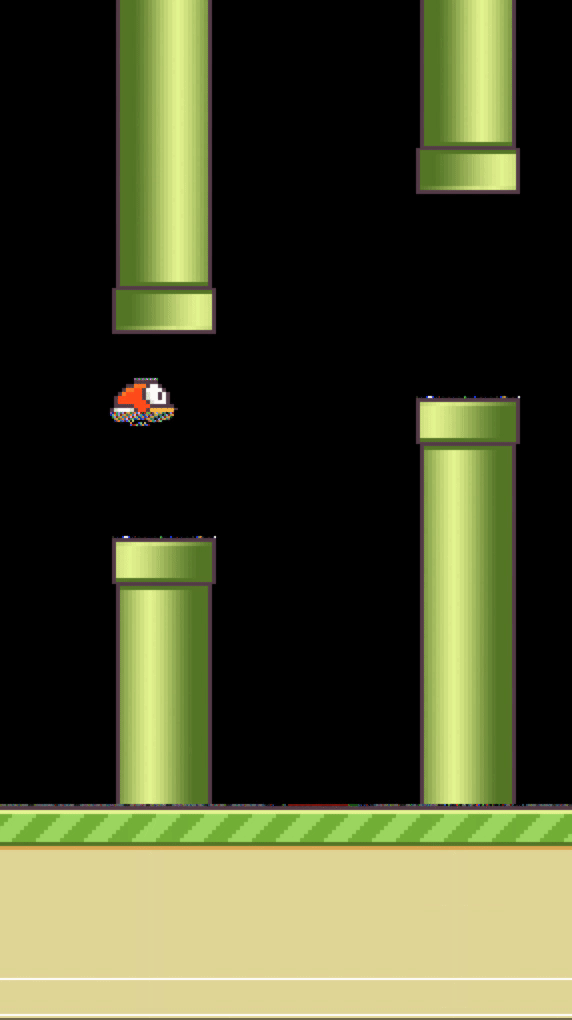
\includegraphics[width=0.8\textwidth]{images/flappybird-0.png}
\caption{Flappybird in Python, \href{images/flappybird.gif}{Animation}}
\end{figure}
\end{column}

\begin{column}[c]{0.75\columnwidth}
\begin{figure}[htbp]
\centering
\includegraphics[width=1.1\textwidth]{images/dot_success.pdf}
\caption{Workflow}
\end{figure}
\end{column}
\end{columns}
\end{frame}

\begin{frame}[label={sec:orge391e48},fragile]{Comp. modeling with HPC using FOSS packages}
 \begin{block}{Fluid dynamics using \texttt{DEDALUS}}
\begin{center}

\includegraphics[width=0.4\textwidth]{images/kh_swirl.jpg}
\end{center}
\end{block}

\begin{columns}
\begin{column}{0.52\columnwidth}
\begin{block}{Solid mech.	using \texttt{Fenics}}
\begin{center}
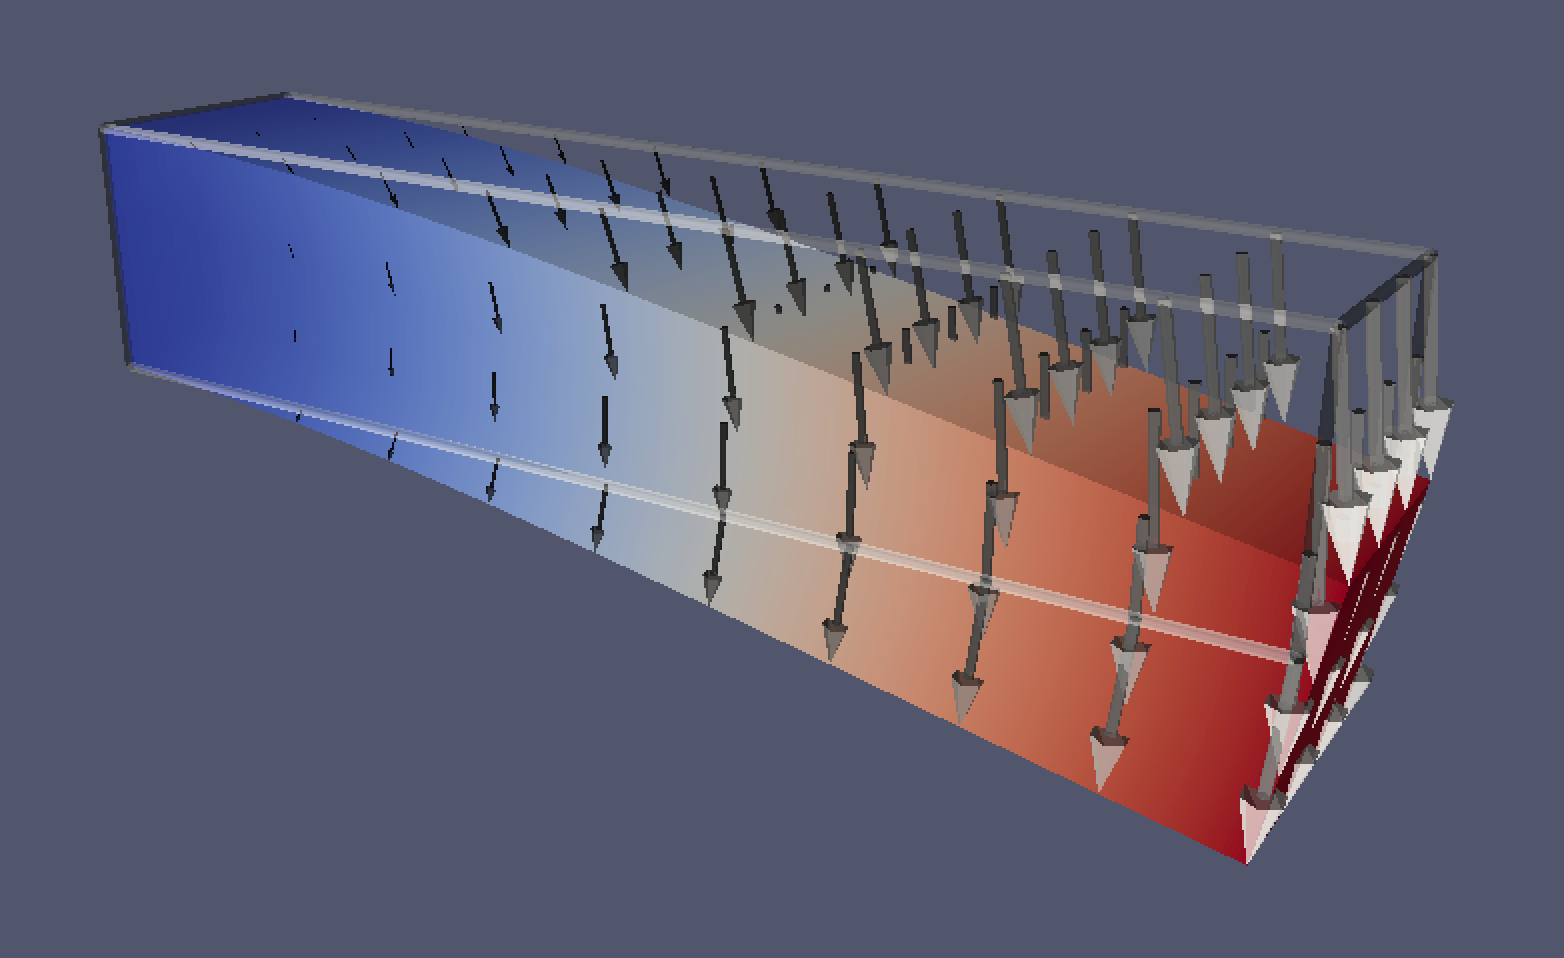
\includegraphics[width=0.8\textwidth]{images/elasticity.png}
\end{center}
\end{block}
\end{column}

\begin{column}{0.5\columnwidth}
\begin{block}{MD using \texttt{ESPResSo}}
\begin{center}
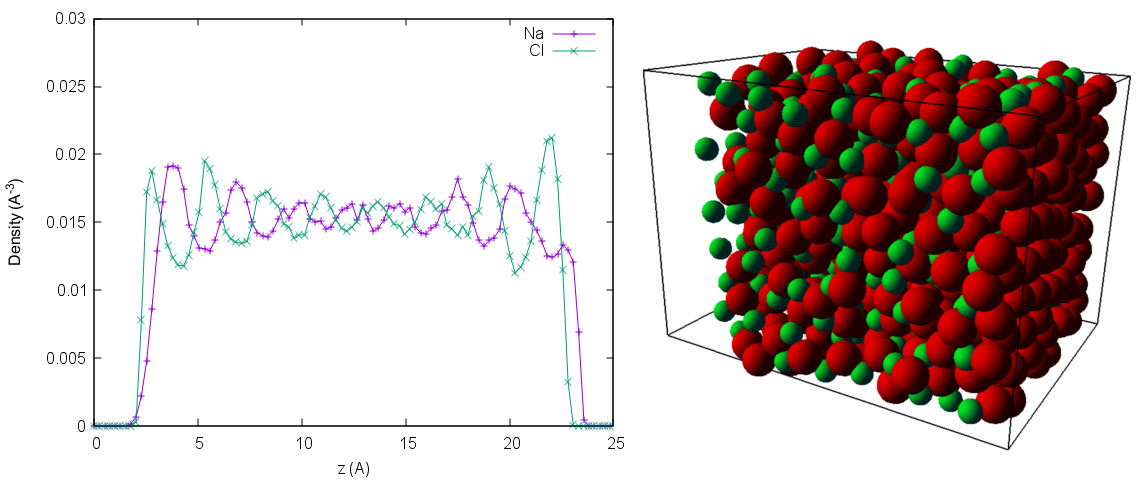
\includegraphics[width=0.9\textwidth]{images/nacl.jpg}
\end{center}
\end{block}
\end{column}
\end{columns}
\end{frame}

\begin{frame}[label={sec:org81f6df2}]{Your favorite applications use Python!}
\begin{itemize}
\item Dropbox
\item Spotify
\item Email clients
\item You name it!
\item An example close to home : \href{code/clangformat.cpp}{ST3 demo}
\end{itemize}
\end{frame}

\begin{frame}[label={sec:org5ae6b1b},fragile]{We will use python for\footnote{\href{https://zulko.github.io/blog/2014/11/13/things-you-can-do-with-python-and-pov-ray/\#disqus\_thread}{Vapory/Povray}}\textsuperscript{,}\,\footnote{\href{http://mattia-lab.com/work/soft-filaments/}{Mattialab}}}
 \begin{itemize}
\item Modeling (\texttt{numpy}, \texttt{scipy})
\item Optimization (\texttt{numpy}, \texttt{scipy})
\item File I/O (\texttt{os}, \texttt{pandas}, \texttt{cereal})
\item Visualization (\texttt{matplotlib}, \texttt{seaborn}, \texttt{povray}, \texttt{vapory})
\end{itemize}
\end{frame}

\section{Introduction to Shell}
\label{sec:org3c848ee}
\begin{frame}[label={sec:org3e77c44}]{Shell?}
\begin{itemize}
\item User interface for access to an operating system's services
\item You have already used it
\begin{itemize}
\item Windows (Desktop, Taskbar, Menu)
\item MacOS (Finder, Dock)
\item \ldots{}
\end{itemize}
\item These are GUI shells
\item We will use CLI (Command line interface) shells here.
\item Idea: Type in commands to perform desired operations.
\end{itemize}
\end{frame}

\begin{frame}[label={sec:org17634d6},fragile]{On to your shell}
 \begin{itemize}
\item MacOS : Find \texttt{Terminal} in \texttt{Applications/Utilities/Terminal} (Spotlight
works too)
\item Ubuntu environments: Type \texttt{terminal} in the dash and select the app.
\item Windows : You can either use \texttt{Command Prompt/Powershell}, but neither of
these support *nix based shells (\texttt{sh/bash/zsh}).
\item If you can't open a terminal session now, worry not. Go to
\url{https://rootnroll.com/d/fish-shell/}.
\end{itemize}
\end{frame}

\begin{frame}[label={sec:org8d891d8},fragile]{Shell demo}
 \begin{block}{Command line is great for code development, but can be a bit intimidating at first.}
\end{block}
Let's go through some of the important ones!

\begin{block}{Design}
\texttt{command [options] argument}
\end{block}
\alert{Demo: Navigating your shell}

If you get stuck:
\begin{itemize}
\item Google is your friend!
\item Use \texttt{whatis <command\_name>} to see a one-line description \alert{Demo}
\item Use \texttt{man <command\_name>} to see all possible options \alert{Demo}
\end{itemize}
\end{frame}

\begin{frame}[label={sec:orga67f4bc},fragile]{View current directory}
 \begin{block}{Command}
\begin{minted}[]{shell}
ls # LiSt directory contents
# tip: -l lists, -a shows all files
\end{minted}
\end{block}

\alert{Output}
\begin{center}
\begin{tabular}{l}
\toprule
01\_intro.org\\
01\_intro.pdf\\
01\_intro.synctex.gz\\
01\_intro.tex\\
\_minted-01\_intro\\
auto\\
code\\
images\\
shell\_example\\
shell\_example.zip\\
show\_me\_to\_the\_class.txt\\
temp\\
\bottomrule
\end{tabular}
\end{center}
\end{frame}

\begin{frame}[label={sec:orged09af5},fragile]{My current directory structure?}
 \begin{block}{Command}
\begin{minted}[]{fish}
tree -d # Visualize directory as a TREE
\end{minted}
\end{block}

\alert{Output}
\tiny
\begin{center}
\begin{tabular}{lllll}
\toprule
. &  &  &  & \\
├── & \_minted-01\_intro &  &  & \\
├── & auto &  &  & \\
├── & code &  &  & \\
│   & ├── & \_\_pycache\_\_ &  & \\
│   & ├── & learn-pandas &  & \\
│   & │   & ├── & data$\backslash$ & games\\
│   & │   & ├── & lessons & \\
│   & │   & │   & └── & DataFiles\\
│   & │   & └── & notebooks & \\
│   & └── & teach\_python\_in\_notebooks &  & \\
│   & ├── & data &  & \\
│   & ├── & figures &  & \\
│   & └── & files &  & \\
│   & └── & images &  & \\
├── & images &  &  & \\
├── & shell\_example &  &  & \\
│   & ├── & src\_code &  & \\
│   & │   & └── & assets & \\
│   & │   & ├── & audio & \\
│   & │   & └── & sprites & \\
│   & └── & story\_books &  & \\
│   & └── & thursday &  & \\
└── & temp &  &  & \\
23 & directories &  &  & \\
\bottomrule
\end{tabular}
\end{center}
\end{frame}

\begin{frame}[label={sec:orgecb288f},fragile]{What's my current directory?}
 \begin{block}{Command}
\begin{minted}[]{shell}
pwd # What is the Present Working Directory?
\end{minted}
\end{block}

\alert{Output}
\tiny
\begin{verbatim}
/Users/tp5/Desktop/Masters_Resources/teaching/ME498_CMO/lectures/01_intro
\end{verbatim}
\end{frame}

\begin{frame}[label={sec:org79718e6},fragile]{Navigate to another directory}
 \begin{block}{Command}
\begin{minted}[]{shell}
cd images # Change Directory
echo "Dir:"
pwd # What is the Present Working Directory?
echo "Contents:"
ls # List contents of the `images` directory
\end{minted}
\end{block}

\alert{Output}
\tiny
\begin{center}
\begin{tabular}{l}
\toprule
Dir:\\
/Users/tp5/Desktop/Masters\_Resources/teaching/ME498\_CMO/lectures/01\_intro/images\\
Contents:\\
dot\_success.pdf\\
elasticity.png\\
flappybird-0.png\\
flappybird.gif\\
format\_method\_keyword\_parameters.png\\
format\_method\_positional\_parameters.png\\
function\_def.png\\
hanoi.jpeg\\
helloworld.png\\
inverse\_design.pdf\\
kh\_swirl.jpg\\
nacl.jpg\\
normalgraph.eps\\
python\_numerics.png\\
so-projections.png\\
svgphp-normal-probability-distribution-14-s1.svg\\
toh\_sol.png\\
vector\_base.eps\\
while\_loop.png\\
while\_loop\_with\_else.png\\
while\_loop\_with\_else\_break.png\\
\bottomrule
\end{tabular}
\end{center}
\end{frame}

\begin{frame}[label={sec:org6f69751},fragile]{Navigate back to source directory}
 \begin{block}{Command}
\begin{minted}[]{shell}
cd images # Change Directory
cd .. # Change Directory to parent directory
# . is present directory
# .. is previous directory
ls # List contents of the parent directory
\end{minted}
\end{block}

\alert{Output} (Same as a couple of slides before)
\scriptsize
\begin{center}
\begin{tabular}{l}
\toprule
01\_intro.org\\
01\_intro.pdf\\
01\_intro.synctex.gz\\
01\_intro.tex\\
\_minted-01\_intro\\
auto\\
code\\
images\\
shell\_example\\
shell\_example.zip\\
show\_me\_to\_the\_class.txt\\
temp\\
\bottomrule
\end{tabular}
\end{center}
\end{frame}

\begin{frame}[label={sec:org070b46d},fragile]{Make a new directory}
 \begin{block}{Command}
\begin{minted}[]{shell}
mkdir MyFolderName # MaKe DIRectory
#-p MaKes intermediate DIRs too
mkdir -p fx/gx/hx
tree -d # List directories as TREE
\end{minted}
\end{block}

\alert{Output} (Same as a couple of slides before)
\tiny
\begin{center}
\begin{tabular}{lllll}
\toprule
. &  &  &  & \\
├── & MyFolderName &  &  & \\
├── & \_minted-01\_intro &  &  & \\
├── & auto &  &  & \\
├── & code &  &  & \\
│   & ├── & \_\_pycache\_\_ &  & \\
│   & ├── & learn-pandas &  & \\
│   & │   & ├── & data$\backslash$ & games\\
│   & │   & ├── & lessons & \\
│   & │   & │   & └── & DataFiles\\
│   & │   & └── & notebooks & \\
│   & └── & teach\_python\_in\_notebooks &  & \\
│   & ├── & data &  & \\
│   & ├── & figures &  & \\
│   & └── & files &  & \\
│   & └── & images &  & \\
├── & fx &  &  & \\
│   & └── & gx &  & \\
│   & └── & hx &  & \\
├── & images &  &  & \\
├── & shell\_example &  &  & \\
│   & ├── & src\_code &  & \\
│   & │   & └── & assets & \\
│   & │   & ├── & audio & \\
│   & │   & └── & sprites & \\
│   & └── & story\_books &  & \\
│   & └── & thursday &  & \\
└── & temp &  &  & \\
27 & directories &  &  & \\
\bottomrule
\end{tabular}
\end{center}
\end{frame}

\begin{frame}[label={sec:orgc81a29d},fragile]{Remove directories and files}
 \begin{block}{Command}
\begin{minted}[]{shell}
rmdir MyFolderName #ReMove DIRectory
rmdir -p fx/gx/hx #same as mkdir
# Caveat : Only does it if the DIR is empty
tree -d
\end{minted}
\end{block}

\alert{Output} (Same as a couple of slides before)
\tiny
\begin{center}
\begin{tabular}{lllll}
\toprule
. &  &  &  & \\
├── & \_minted-01\_intro &  &  & \\
├── & auto &  &  & \\
├── & code &  &  & \\
│   & ├── & \_\_pycache\_\_ &  & \\
│   & ├── & learn-pandas &  & \\
│   & │   & ├── & data$\backslash$ & games\\
│   & │   & ├── & lessons & \\
│   & │   & │   & └── & DataFiles\\
│   & │   & └── & notebooks & \\
│   & └── & teach\_python\_in\_notebooks &  & \\
│   & ├── & data &  & \\
│   & ├── & figures &  & \\
│   & └── & files &  & \\
│   & └── & images &  & \\
├── & images &  &  & \\
├── & shell\_example &  &  & \\
│   & ├── & src\_code &  & \\
│   & │   & └── & assets & \\
│   & │   & ├── & audio & \\
│   & │   & └── & sprites & \\
│   & └── & story\_books &  & \\
│   & └── & thursday &  & \\
└── & temp &  &  & \\
23 & directories &  &  & \\
\bottomrule
\end{tabular}
\end{center}
\end{frame}

\begin{frame}[label={sec:orgee2a471},fragile]{If the directory has files, then}
 \begin{block}{Command}
\begin{minted}[]{bash}
mkdir MyFolderName
# Creates a dummy txt file
touch MyFolderName/test.txt
# rmdir does not work, as it needs empty DIR
# Use rm instead with -r:recursive, -f:force
rm -rf MyFolderName
tree -d
\end{minted}
\end{block}

\alert{Output} (Same as a couple of slides before)
\tiny
\begin{center}
\begin{tabular}{lllll}
\toprule
. &  &  &  & \\
├── & \_minted-01\_intro &  &  & \\
├── & auto &  &  & \\
├── & code &  &  & \\
│   & ├── & \_\_pycache\_\_ &  & \\
│   & ├── & learn-pandas &  & \\
│   & │   & ├── & data$\backslash$ & games\\
│   & │   & ├── & lessons & \\
│   & │   & │   & └── & DataFiles\\
│   & │   & └── & notebooks & \\
│   & └── & teach\_python\_in\_notebooks &  & \\
│   & ├── & data &  & \\
│   & ├── & figures &  & \\
│   & └── & files &  & \\
│   & └── & images &  & \\
├── & images &  &  & \\
├── & shell\_example &  &  & \\
│   & ├── & src\_code &  & \\
│   & │   & └── & assets & \\
│   & │   & ├── & audio & \\
│   & │   & └── & sprites & \\
│   & └── & story\_books &  & \\
│   & └── & thursday &  & \\
└── & temp &  &  & \\
23 & directories &  &  & \\
\bottomrule
\end{tabular}
\end{center}
\end{frame}

\begin{frame}[label={sec:org7031c06},fragile]{See file contents}
 \begin{block}{Command}
\begin{minted}[]{sh}
# Print out contents of a file
cat show_me_to_the_class.txt
# Concatenate And prinT
\end{minted}
\end{block}

\alert{Output}
\small
\begin{verbatim}
I am a file whose contents the class needs to see.
\end{verbatim}
\end{frame}

\begin{frame}[label={sec:orgd76731a},fragile]{Move files around}
 \begin{block}{Command}
\begin{minted}[]{sh}
# MoVe a file, similar to cut/paste
# prototype: mv src target
# Can also move into different folders
mv show_me_to_the_class.txt dont_show_me.txt
ls
mv dont_show_me.txt show_me_to_the_class.txt
\end{minted}
\end{block}

\alert{Output}
\tiny
\begin{center}
\begin{tabular}{l}
\toprule
01\_intro.org\\
01\_intro.pdf\\
01\_intro.synctex.gz\\
01\_intro.tex\\
\_minted-01\_intro\\
auto\\
code\\
dont\_show\_me.txt\\
images\\
shell\_example\\
shell\_example.zip\\
temp\\
\bottomrule
\end{tabular}
\end{center}
\end{frame}

\begin{frame}[label={sec:org1d03938},fragile]{Copy files around}
 \begin{block}{Command}
\begin{minted}[]{sh}
# CoPy a file, similar to copy/paste
# prototype: cp src target
# Can also move into different folders
cp show_me_to_the_class.txt dont_show_me.txt
ls
\end{minted}
\end{block}

\alert{Output}
\tiny
\begin{center}
\begin{tabular}{l}
\toprule
01\_intro.org\\
01\_intro.pdf\\
01\_intro.synctex.gz\\
01\_intro.tex\\
\_minted-01\_intro\\
auto\\
code\\
dont\_show\_me.txt\\
images\\
shell\_example\\
shell\_example.zip\\
show\_me\_to\_the\_class.txt\\
temp\\
\bottomrule
\end{tabular}
\end{center}
\end{frame}

\begin{frame}[label={sec:org1ad4523},fragile]{Launch applications}
 \begin{block}{Command}
\begin{minted}[]{bash}
# Do we have Python?---the which command
which python3
# Let's launch this python3 from shell
python3 -c 'print("Hello_world_from_ME498")'
# Full disclosure : Location of the Python
# executable has to be in your PATH variable
\end{minted}
\end{block}

\alert{Output}
\small
\begin{center}
\begin{tabular}{l}
\toprule
/usr/local/bin/python3\\
Hello\_world\_from\_ME498\\
\bottomrule
\end{tabular}
\end{center}
\end{frame}

\begin{frame}[label={sec:orgfef3cdd}]{More about your shell}
\begin{itemize}
\item We have just scratched the surface in exploring the capabilities of the
shell
\item Here's a \href{http://www.ee.surrey.ac.uk/Teaching/Unix/}{highly recommended gentle tutorial }\footnote{\url{http://www.ee.surrey.ac.uk/Teaching/Unix/}}  to some essential
commands
\end{itemize}
\end{frame}

\section{Introduction to Python}
\label{sec:org6669157}
\begin{frame}[label={sec:org981ed58},fragile]{Outline\footnote{\url{https://www.python-course.eu/python3\_course.php}}}
 \begin{itemize}
\item Help you setup \texttt{Python}
\item Basics of \texttt{Python} as a programming language
\begin{itemize}
\item \texttt{Python} interactive shell and launching scripts
\item Data types and operations: Common types, lists, dicts
\item Conditionals and loops, iterators
\item Functions and recursion
\item Basic I/O
\item Classes?
\item Modules and packages
\end{itemize}
\end{itemize}
\note{:B\_note:
\begin{itemize}
\item Any cribs/complaints?
\item How's shell? Finding it hard?
\item Example for use: \url{https://github.com/ftakie2/echo360Scrapper}
\end{itemize}}
\end{frame}

\begin{frame}[label={sec:org27a0879},fragile]{Installation/Setup}
 \begin{itemize}
\item Fetch the install instructions at Compass (Setup -> 00\_setup\_basics.pdf) and follow it.
\item Try and perform the OS agnostic steps in the install instructions first,
for the purposes of learning Python in today's lecture.
\item If you still can't get it setup, use a cloud-based REPL (\texttt{repl.it, onlinegdb.com})
\item What is : \texttt{Python}, \texttt{Python3}, \texttt{pip}, \texttt{conda}, \texttt{easy\_install}, \texttt{jupyter}
\item (Logistics) Exercises will be prescribed in the form of \texttt{jupyter} notebooks
\end{itemize}
\end{frame}

\begin{frame}[label={sec:org8cdf352},fragile]{Python interactive shell}
 \note{:B\_note:
\begin{itemize}
\item Ask them if all variable names work\ldots{} for example 2ducks = 2
\item \textasciitilde{}and, as, assert, break, class, continue, def, del, elif, else, except,
\end{itemize}
exec, finally, for, from, global, if, import, in, is, lambda, not, or,
pass, print, raise, return, try, while, with, yield\textasciitilde{}
\begin{itemize}
\item EXERCISE : ::inexact arithmetic--Python: 0.1+0.2 = 0.3? Show matlab
\item Python 3: 1/3 = 0.3333. Switch to Python2 gotcha. Show that 1/3 is 0;
\item Addition of strings ``hello'' + ``wprld''
\item EXERCISE : given x, find 4.3 x**4 - 3.2x**3 + 2.1x**2 - 1.0x + 10.0
\end{itemize}}
\alert{Demo}
\begin{itemize}
\item Hello world, \texttt{print("Hello world")}
\item Quit shell, \texttt{quit()} or \texttt{Ctrl + D}
\item Calculator, \texttt{35.9*42.1}
\item Variables, \texttt{x = 42}
\item Special variable \texttt{\_}
\item Strings, \texttt{my\_str="This is my\_str"}
\item Comments, \texttt{\# I am a comment}
\item Getting help using \texttt{help()}
\end{itemize}
\end{frame}
\begin{frame}[label={sec:org1716a3d},fragile]{Python scripts}
 \note{:B\_note:
\begin{itemize}
\item Imports are a way to ``use'' the file and definitions inside a file. Similar
to \#include directives.
\item Interactive: Make them do the import and see the folder
\item Explain bytecode of helloworld
\end{itemize}}
\alert{Demo}
\begin{itemize}
\item Hello world from the file \texttt{hello\_world.py}
\item ``Import'' \texttt{hello\_world.py}
\item \texttt{\_\_pycache\_\_}?
\end{itemize}
\end{frame}

\begin{frame}[label={sec:org3e95e7d},fragile]{Common types and operations}
 \note{:B\_note:
\begin{itemize}
\item SKIP---id as a function to see address before copy
\item type()---say that its a function that helps us see what type a value is
\item the bin, hex commands for converting ints
\item Conversion of float into int and int into float
\item Show +, - , \alert{\alert{, / and *}} for floats + ints
\item Additionally show // for ints and floats
\end{itemize}}
\alert{Demo}
\begin{itemize}
\item \texttt{type()}
\item Integers, \texttt{x=42} or \texttt{x=0b101010}
\item Floating point numbers, \texttt{f=42.12} or \texttt{f=2.718281828459045}
\item Complex numbers, \texttt{c=2.06 + 5.23j}
\item The operations \texttt{+, - , * , /, // and  **}
\item Copying common types
\end{itemize}
\end{frame}

\begin{frame}[label={sec:org938ab8d},fragile]{Common types and operations contd.}
 \note{:B\_note:
\begin{itemize}
\item Interactive: Make sure the indexing is understood [f,l), especially MATLAB users
\item Demo. Construct the following strings:
\item ImLearningPythonNow | ningPyth | ningAPyth
\item a = ImLearningPythonNow
\item b = ningPyth. The answer is a[6:14]
\item a.find('n') and a.find('h'). These are methods acting on variables (Use TAB
and show them)
\item c = ningAPyth. The answer
\item c = a[6:10] + 'A' + a[10:14]. See continuity in loop indexing
\end{itemize}}
\alert{Demo}
\begin{itemize}
\item Strings, \texttt{x="42"} or \texttt{x='42'}
\item Backslash for special characters, \texttt{my\_str ='What\textbackslash{}'s that?'}
\item Multiline strings (triple quotes), \texttt{my\_str=''' How's that'''}
\item \texttt{t = "Hello World"} indexed as
\end{itemize}
\begin{center}
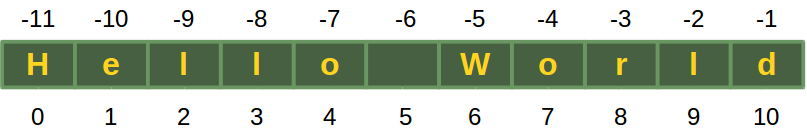
\includegraphics[width=.9\linewidth]{images/helloworld.png}
\end{center}
\begin{itemize}
\item \(\therefore\) \texttt{t[0] = 'H', t[6]='W', t[-3]='r'}
\item Operations \texttt{len(), +, *, [], [:]}
\end{itemize}
\end{frame}

\begin{frame}[label={sec:org348134b},fragile]{Some more operations}
 \note{:B\_note:
\begin{itemize}
\item my\_str = 'saudi' ; 'a' in my\_str returns True
\item 2 and 3 returns 3 as 2 evalutes to True (ask people who know Python
already)
\item 0 and 3? returns 0.
\item Same for 2 or 3 and 0 or 1.
\item Precedence order! 3 and 5 and 9 or 2 and 4 or 5
\item Link precendence logically to the practice sheet!
\end{itemize}}
\alert{Demo}
\begin{itemize}
\item Boolean: \texttt{True, False}
\item \texttt{in}
\item \texttt{or, and}
\item Comparison \texttt{<,>,==}
\end{itemize}
\end{frame}

\begin{frame}[label={sec:orgfd95942},fragile]{Practice}
 \begin{block}{Please attempt}
\texttt{02\_datatypes\_strings\_numbers\_and\_variables.ipynb}
\end{block}
\begin{itemize}
\item Brief demo on how to access and run notebooks\ldots{}
\item \texttt{00\_introduction\_to\_notebooks.ipynb} will be uploaded, and is not compulsary
\end{itemize}
\note{:B\_note:
\begin{itemize}
\item Run keycastr
\item show command + enter for running scripts
\item Show ? for doc. Tab for completion. Shift + Tab for online docs
\end{itemize}}
\end{frame}

\begin{frame}[label={sec:org46ab2fd},fragile]{Sequential types}
 \begin{itemize}
\item Strings, \alert{Lists} and \alert{Tuples} (and \alert{\emph{sets}})
\item Underlying concepts (and hence operations) are the same. So know one
\(\rightarrow\) know all!
\item Lists are ``an ordered group of items or elements''.
\item Are like arrays in \texttt{C, C++, Java}, but are more powerful*
\item Tuples are immutable lists
\end{itemize}
\end{frame}

\begin{frame}[label={sec:org7ef2a8b},fragile]{Lists}
 \note{:B\_note:
\begin{itemize}
\item Say that for list, I'll show you examples and code some lists and show
operations on lists
\item Use type to see the object type of the list
\item Then have a small activity
\item Say you'll understand why its powerful
\item Then homework
\end{itemize}}
To create a list:
\begin{minted}[]{python}
my_list = [42, 'kat', 10.24, "meow"]
\end{minted}

Features:
\begin{itemize}
\item Are ordered (Order does not change)
\item May contain arbitrary objects (See example above)
\item Elements of a list can be accessed by an index (\texttt{my\_list[0]=42})
\item They are arbitrarily nestable (they can contain other lists as sublists)
\item Variable size (can add/remove items from lists)
\item They are mutable (the elements of a list can be changed)
\end{itemize}
\end{frame}
\begin{frame}[label={sec:org90d39e8},fragile]{Examples of lists}
 \begin{center}
\begin{tabular}{ll}
\toprule
List & Description\\
\midrule
\texttt{[]} & An empty list\\
\texttt{[1,1,2,3,5,8]} & A list of integers\\
\texttt{[42, "Whasup?", 3.1415]} & A list of mixed types\\
\texttt{["NY", "Philly", "Boston"]} & A list of Strings\\
\texttt{[["Chmp",61820], ["Urb",61801]]} & A nested list\\
\bottomrule
\end{tabular}
\end{center}
\end{frame}

\begin{frame}[label={sec:org6d30c50},fragile]{Operations on lists}
 \note{:B\_note:
\begin{itemize}
\item Construct a bigass list. 8 or 9 elements say. Break a string down using
split and add using the + operator!
\item Show len and *. Access one member using a[4] say.
\item Demo in slicing, negative indices as well, a[2:5], a[2:], a[2:-1], a[-3:]
\item a[:2:-1] (say)
\item Construct sublist by using the above composition
\item Sublist indexing show [0][1]
\end{itemize}}
\alert{Demo}, similar to strings
\begin{itemize}
\item Operations \texttt{len(), +, *, []} and \texttt{[:]} (slicing)
\item \texttt{seq[begin: end: step]}
\item \texttt{in, not in} for checking elements
\item Comparison
\item Sublists indexing
\end{itemize}
\end{frame}

\begin{frame}[label={sec:org228a8a4},fragile]{Additional operations on lists}
 \note{:B\_note:
\begin{itemize}
\item demo pop(i) to pop at the ith location
\item pop() at empty list? IndexError (Exceptions\ldots{}won't get to that)
\item Motivate need for extend by showing why append fails (append list say)
\item Insert (index, elem)
\item remove() if not found? ValueError
\end{itemize}}
\alert{Demo}, unique to lists
\begin{itemize}
\item \texttt{pop}
\item \texttt{append}
\item \texttt{extend} (for appending any iterable)
\item \texttt{index} (find first matching index)
\item \texttt{insert} (at any location)
\item \texttt{remove} (first found element)
\end{itemize}
\end{frame}
\begin{frame}[label={sec:orgd44b69a},fragile]{Activity}
 \note{:B\_note:
\begin{itemize}
\item str=``Python 3 is awesome dude''; a = str.split(); a[1]=float(a[1]);
\item b=a[0:3]*2; b.pop(); b[-1]=int(b[-1])
\item c=b.copy(); c.append('?'); c.insert(3,'not')
\item d=[``yes'', ``it'', ``is?'']
\item c.extend(d). Why not +=? Efficiency! extend does it inplace?
\item c.remove(``not'')
\end{itemize}}
Give me the following lists, minimal keystroke:
\begin{itemize}
\item \texttt{a = ['Python', 3.0, 'is', 'awesome', 'dude']}
\item \texttt{b = ['Python', 3.0, 'is', 'Python', 3]}
\item \texttt{c = ['Python', 3.0, 'is', 'not', 'Python', 3, '?']}
\item \texttt{d = ['Yes', 'it', 'is']}
\item \texttt{c = ['Python', 3.0, 'is', 'not', 'Python', 3, '?', 'Yes, 'it, 'is']}
\item \texttt{e = ['Python', 3.0, 'is', 'Python', 3, '?', 'Yes, 'it, 'is']}
\end{itemize}
\texttt{[begin: end: step], pop, append, extend, index, insert, remove}
\end{frame}
\begin{frame}[label={sec:orgdd29a79},fragile]{Tuples (very briefly)}
 \begin{itemize}
\item Immutable list---\alert{cannot be changed in any way once it has been created}
\item Nice for \emph{constness} and speed
\item Create one as follows
\footnotesize
\begin{minted}[]{python}
my_tuple = ("tuples", "are like", "immutable", "lists")
\end{minted}
\end{itemize}

\begin{itemize}
\item \alert{Demo} cannot change/add/remove elements
\end{itemize}
\end{frame}
\begin{frame}[label={sec:org5c55c41},fragile]{Copies of lists}
 \note{:B\_note:
\begin{itemize}
\item Ask them to do list copy and see whether one can modify another
\item x,y. y=x. show id(x,y)
\item Change value of y and show id
\item Do the same for lists and show id()
\item Slicing or copy changes id
\item Deepcopy to do sublists
\end{itemize}}
\begin{itemize}
\item \alert{Demo} Understanding copies of variables using \texttt{id()}
\item \texttt{Python} creates copies only if we \alert{explicitly demand} it.
\item \alert{Demo} \texttt{=} operation on lists
\item Inplace transforms creates \emph{references}
\item Use slice / \texttt{copy()} method as a workaround (Shallow copy)
\item \alert{Demo} Doesn't work for sublists. Use Deep copy.
\end{itemize}
\end{frame}

\begin{frame}[label={sec:org88cda9b},fragile]{Numerical lists}
 \note{:B\_note:
\begin{itemize}
\item Note same concept [forst, last)
\item You have bunch more of such functions like min and max. To know all about
them do practice..
\end{itemize}}
\begin{itemize}
\item \texttt{range} can generate numerical lists
\begin{minted}[]{python}
# Store the first ten numbers in a list.
numbers = list(range(1,11))
print((numbers))
\end{minted}

\begin{verbatim}
[1, 2, 3, 4, 5, 6, 7, 8, 9, 10]
\end{verbatim}

\item \texttt{min(), max(), sum()} functions
\begin{itemize}
\item \texttt{min(numbers)} prints \texttt{1}
\item \texttt{max(numbers)} prints \texttt{10}
\item \texttt{sum(numbers)} prints \texttt{55}
\end{itemize}
\end{itemize}
\end{frame}
\begin{frame}[label={sec:orge6ed5f4},fragile]{Practice}
 \begin{block}{Please attempt}
\texttt{03\_lists\_tuples\_and\_sets.ipynb}
\end{block}
\end{frame}

\begin{frame}[label={sec:orge68ae69},fragile]{Dictionaries}
 \note{:B\_note:
\begin{itemize}
\item Use type to see the object type
\item Ask them to try out immutability of keys---need them!
\end{itemize}}
\begin{itemize}
\item \texttt{Python}'s associative arrays---basically has key-value pairs
\item Initialize dictionary like so:
\footnotesize
\begin{minted}[]{python}
# Create a dictionary
food = {"ham" : "yes", "egg" : "yes", "spam" : "no" }
print(food)
print(food["ham"]) # Returns the value
food["spam"] = "yes" # Change the value
print(food)
\end{minted}
\end{itemize}


\begin{itemize}
\item What about mutability of keys?

\item ---OUTPUT---
\footnotesize
\begin{verbatim}
{'ham': 'yes', 'egg': 'yes', 'spam': 'no'}
yes
{'ham': 'yes', 'egg': 'yes', 'spam': 'yes'}
\end{verbatim}
\end{itemize}
\end{frame}

\begin{frame}[label={sec:org4bccf4b},fragile]{Operations on dictionaries}
 \note{:B\_note:
\begin{itemize}
\item Use (key, value) = pop(key) or popitem
\item Demonstrate empty dict pop
\item Ask given the knowledge of what happended in list, what do they think will
happen in dict? a=d? a.clear(); a? d?
\item Update()---create only unique! Show example with redundant list. Something
like a; b=a.copy(); Change one value in b; a.update(b) updates value.
\item But if b is different, a.update(b) adds key/value pairs or updates values
\end{itemize}}
\alert{Ans}---Keys need to be immutable.

\alert{Demo}
\begin{itemize}
\item \texttt{len()}
\item \texttt{del d[key]}
\item \texttt{k in/not in d}
\item \texttt{pop(key)/popitem} (Last key removal)
\item \texttt{copy} (shallow copy)
\item \texttt{clear} (removes all key-value pairs)
\item \texttt{update} (Merge dictionaries)
\end{itemize}
\end{frame}
\begin{frame}[label={sec:orgb41616b},fragile]{Conditional statements}
 \begin{itemize}
\item Decisions, decisions, decisions
\item \texttt{if}, \texttt{if-else}, \texttt{if-elif-else}
\tiny
\begin{minted}[]{python}
# Example if
    # Note you dont need brackets like if(True):
if True:
    print("This block gets executed")

# Example if-else
if 5==5:
    print("This block gets executed")
else:
    print("This block doesn't get executed")

# Example if-else-if
a = 2
if a==2:
    print("If block")
    a = 3
elif a==3:
        # Should this block run?
    print("Elif block")
else:
    print("Else block")
\end{minted}
\end{itemize}


\begin{itemize}
\item Indentation is key in \texttt{Python} (No \{\}, [] or variants)
\end{itemize}
\end{frame}
\begin{frame}[label={sec:orge0ca941},fragile]{Conditional assignments}
 \note{:B\_note:
\begin{itemize}
\item Can come in a variety of form and shapes that you can only learn if you do
the following ipython notebook
\end{itemize}}
\begin{itemize}
\item Assignments are possible using conditionals
\footnotesize
\begin{minted}[]{python}
# Max of two numbers
a = 4; b = 5;
max_ab = a if (a>b) else b

# Can also use as expression
max_ab = (a if (a>b) else b)*3.14 - 2.718

\end{minted}
\end{itemize}


\begin{itemize}
\item Conditional statements can be used as expressions
\end{itemize}
\end{frame}
\begin{frame}[label={sec:org6a4a87b},fragile]{Practice}
 \begin{block}{Please attempt}
\texttt{04\_if\_statements.ipynb}
\end{block}
\end{frame}

\begin{frame}[label={sec:orgd72e7c8},fragile]{Loops in \texttt{Python}}
 \begin{itemize}
\item Roughly two types:
\begin{itemize}
\item Condition-controlled: Loop repeated until a given condition changes, e.g.
changes from True to False. e.g. \texttt{while}.
\item Collection-controlled: Looping through elements of a ``collection'' (\texttt{list},
\texttt{dict} or ordered sequence). e.g. \texttt{for}.
\end{itemize}
\item Example (What's the output?)
\footnotesize
\begin{minted}[]{python}
# While example---whats the answer?
counter = 1
while counter <= 100:
    counter += 1
print("Counter reaches {}".format(counter))
\end{minted}

\footnotesize
\begin{minted}[]{python}
# For example---whats the answer?
counter = 1
for x in range(100):
    counter += 1
print("Counter reaches {}".format(counter))
\end{minted}
\end{itemize}

\note{:B\_note:
\begin{itemize}
\item While loop == 101
\item For loop == 101
\item Say that we have seen range in a different context before and what is it?
\item Make sure difference between range is known (1-100) and (0-99)
\end{itemize}}
\end{frame}

\begin{frame}[label={sec:orgc707255},fragile]{The \texttt{while} loop \footnote{Picture credits:\href{https://www.python-course.eu/python3\_loops.php}{ Python Course}\label{org6dcf9e0}}}
 \begin{columns}
\begin{column}{0.48\columnwidth}
\scriptsize
\begin{minted}[]{python}
# Print sum of first n numbers
n = 100
s = 0
counter = 1
while counter <= n:
    s = s + counter
    counter += 1
print("Sum of 1 until %d: %d" % (n,s))
\end{minted}

\begin{verbatim}
Sum of 1 until 100: 5050
\end{verbatim}
\end{column}
\begin{column}{0.45\columnwidth}
\footnotesize
\begin{figure}[htbp]
\centering
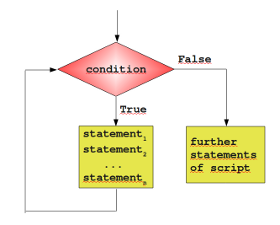
\includegraphics[width=0.8\textwidth]{images/while_loop.png}
\caption{While logic}
\end{figure}
\end{column}
\end{columns}
\end{frame}

\begin{frame}[label={sec:orgfd72dc0},fragile]{The \texttt{while-else} loop?}
 \begin{columns}
\begin{column}{0.48\columnwidth}
\scriptsize
\begin{minted}[]{python}
# Print sum of first n numbers
n = 100
s = 0
counter = 1
while counter <= n:
    s = s + counter
    counter += 1
else:
    print("Why is this needed?")
print("Sum of 1 until %d: %d" % (n,s))
\end{minted}

\begin{verbatim}
Why is this needed?
Sum of 1 until 100: 5050
\end{verbatim}
\end{column}

\begin{column}{0.45\columnwidth}
\footnotesize
\begin{figure}[htbp]
\centering
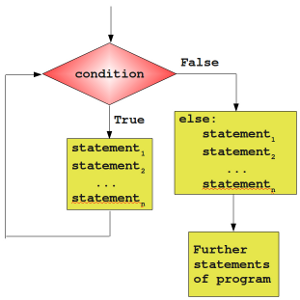
\includegraphics[width=0.8\textwidth]{images/while_loop_with_else.png}
\caption{While-else logic}
\end{figure}
\end{column}
\end{columns}

\note{:B\_note:
\begin{itemize}
\item else part Always gets executed at the end
\item Where do you think it is useful? I mean we could have just put it at the
end with the rest of the stuff no?
\item Thats where our friend break comes in!
\end{itemize}}
\end{frame}
\begin{frame}[label={sec:org68fc734},fragile]{\texttt{break} statement}
 \begin{columns}
\begin{column}{0.48\columnwidth}
\scriptsize
\begin{minted}[]{python}
# Print sum of first n numbers
# Till 100!
n = 100
s = 0
counter = 1
while counter <= n:
    if counter > 50:
        break
    s = s + counter
    counter += 1
else:
    print('''Loop ran for
    all %d iterations''' % (n))
print('''Sum of 1 until %d: %d'''
        % (min((counter-1, n)),s))
# Output below
\end{minted}

\begin{verbatim}
Sum of 1 until 50: 1275
\end{verbatim}
\end{column}


\begin{column}{0.45\columnwidth}
\footnotesize
\begin{figure}[htbp]
\centering
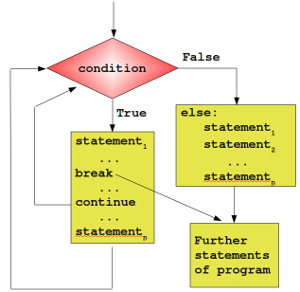
\includegraphics[width=0.8\textwidth]{images/while_loop_with_else_break.png}
\caption{While-else logic}
\end{figure}
\end{column}
\end{columns}
\end{frame}

\begin{frame}[label={sec:orgd836462},fragile]{\texttt{break} statement contd}
 \begin{columns}
\begin{column}{0.48\columnwidth}
\scriptsize
\begin{minted}[]{python}
# Print sum of first n numbers
# Only till 30 now!!!
n = 30
s = 0
counter = 1
while counter <= n:
    if counter > 50:
        break
    s = s + counter
    counter += 1
else:
    print('''Loop ran for
all %d iterations''' % (n))
print('''Sum of 1 until %d: %d'''
    % (min((counter-1, n)),s))
# Output below
\end{minted}

\begin{verbatim}
Loop ran for
all 30 iterations
Sum of 1 until 30: 465
\end{verbatim}
\end{column}

\begin{column}{0.45\columnwidth}
\footnotesize
\begin{figure}[htbp]
\centering
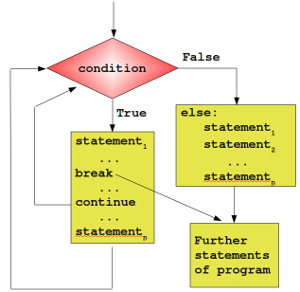
\includegraphics[width=0.8\textwidth]{images/while_loop_with_else_break.png}
\caption{While-else logic}
\end{figure}
\end{column}
\end{columns}
\end{frame}

\begin{frame}[label={sec:org93d11e2},fragile]{\texttt{for} loops}
 \note{:B\_note:
\begin{itemize}
\item for x in b: print(x)---do for lists
\item Question: Does it work on tuples and strings and dicsts
\item Question: But what to do when we wenat index list?  enum?
\item Question: key-value pairs in Dicts? .items()
\item range (begin, end, step) (seen earlier)
\item for x in range(10, 20, 2): print(x)
\end{itemize}}
\begin{itemize}
\item Iterator: Loops over elements of a sequence
\item Syntax:
\scriptsize
\begin{minted}[]{python}
for <variable> in <sequence>:
    <statements>
else:
    <statements>
\end{minted}
\end{itemize}


\begin{itemize}
\item \alert{Demo} Iterating over lists, dicts, tuples and strings
\item \alert{Demo} \texttt{Range} for numbered sequences
\end{itemize}
\end{frame}
\begin{frame}[label={sec:orgfcf7871},fragile]{Activity}
 \note{:B\_note:
}
Write a script that produces the following strings:

\begin{itemize}
\item \texttt{acegikmoqsuwy}
\item \texttt{aCeGiKmOqSuWy}
\item \texttt{BdFhJlNpRtVxZ}
\end{itemize}

\alert{Hints}: consider using \texttt{chr()} and \texttt{ord()} and \texttt{str.upper()} / \texttt{str.lower()}
\end{frame}
\begin{frame}[label={sec:orgfbca6c8},fragile]{\texttt{continue} statement}
 \begin{itemize}
\item In the example below, using a \texttt{break} quits the for loop
\scriptsize
\begin{minted}[]{python}
edibles = ["ham", "spam","eggs","nuts"]
for food in edibles:
    if food == "spam":
        print("No more spam please!")
        break
    print("Great, delicious " + food)
else:
    print("I am so glad: No spam!")
print("Finally, I finished stuffing myself")
# Output below
\end{minted}

\begin{verbatim}
Great, delicious ham
No more spam please!
Finally, I finished stuffing myself
\end{verbatim}
\end{itemize}


\begin{itemize}
\item But what if our disgust with spam is not so high that we want to stop
consuming the other food?
\end{itemize}
\end{frame}

\begin{frame}[label={sec:org246e05a},fragile]{\texttt{continue} statement contd.}
 \begin{itemize}
\item Simple! Replace \texttt{break} with \texttt{continue}
\scriptsize
\begin{minted}[]{python}
edibles = ["ham", "spam","eggs","nuts"]
for food in edibles:
    if food == "spam":
        print("No more spam please!")
        continue # replaces break
    print("Great, delicious " + food)
else:
    print("I am so glad: No spam!")
print("Finally, I finished stuffing myself")
# Output below
\end{minted}

\begin{verbatim}
Great, delicious ham
No more spam please!
Great, delicious eggs
Great, delicious nuts
I am so glad: No spam!
Finally, I finished stuffing myself
\end{verbatim}
\end{itemize}
\end{frame}

\begin{frame}[label={sec:org1b65278},fragile]{Practice}
 \begin{block}{Please attempt}
\texttt{05\_while\_loops\_and\_user\_input.ipynb}
\texttt{06\_dictionaries.ipynb}
\end{block}
\end{frame}

\begin{frame}[label={sec:orgbda64c4},fragile]{Towards functions}
 \begin{itemize}
\item \texttt{Functions} are quintessential to any programming language.
\item Are ``structured elements to group a set of statements so they can be utilized more than once''
\item We have already used a function before: \texttt{print()} !
\end{itemize}
\begin{block}{\texttt{print()} prototype}
\texttt{print(value, ..., sep=' ', end='\textbackslash{}n', file=sys.stdout, flush=False)}
\end{block}
\begin{itemize}
\item Tip: Type \texttt{print?} or \texttt{print} and \texttt{SHIFT+TAB} to view docs in \texttt{ipython}
\item \alert{DEMO}
\end{itemize}
\note{:B\_note:
\begin{itemize}
\item Show multiple arguments: print(a,b,c)
\item Show searation between: print(a,b,c,sep=':)')
\item Show end characters: print(a);print(b, end='\t');print(``c'')
\item show write to file using file: print
\item Explain what flush is\ldots{}but don't go into detail
\end{itemize}}
\end{frame}

\begin{frame}[label={sec:org774caa6},fragile]{Quick detour: How to format output?}
 \begin{itemize}
\item Always use the \texttt{format()} method for formatting strings
\item Positional or keyword params \textsuperscript{\cref{org6dcf9e0}}
\end{itemize}
\begin{center}
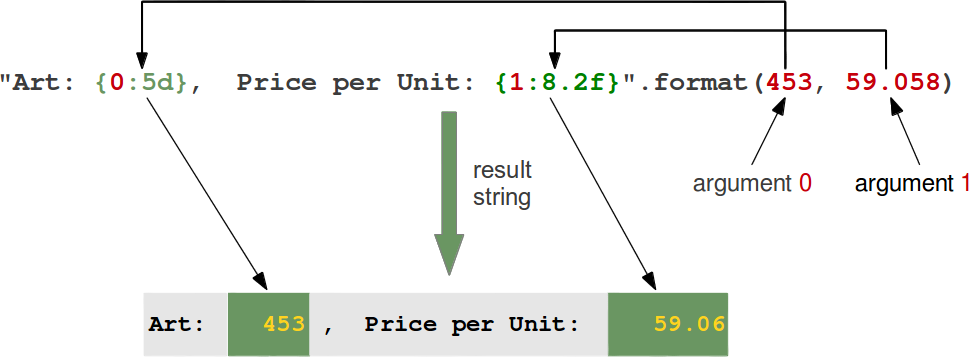
\includegraphics[width=0.7\textwidth]{images/format_method_positional_parameters.png}
\end{center}
\begin{itemize}
\item There are many other formatting tools too! \footnote{\href{https://www.python-course.eu/python3\_formatted\_output.php}{Formatting output. Python Course}}
\item \alert{DEMO}
\end{itemize}
\note{:B\_note:
\begin{itemize}
\item Ask people to play around with formatting shown on the screen
\item Show float and int formatting
\item Show \{:06d\}z ero fill
\item Show \{:<20s\} < and > for right and left fill and \^{} for centered
\end{itemize}}
\end{frame}

\begin{frame}[label={sec:org1914fc3}]{Functions}
\begin{itemize}
\item Syntax \footnote{\href{http://hcc-cs.weebly.com/functions.html}{HCC-CS}}
\end{itemize}
\begin{center}
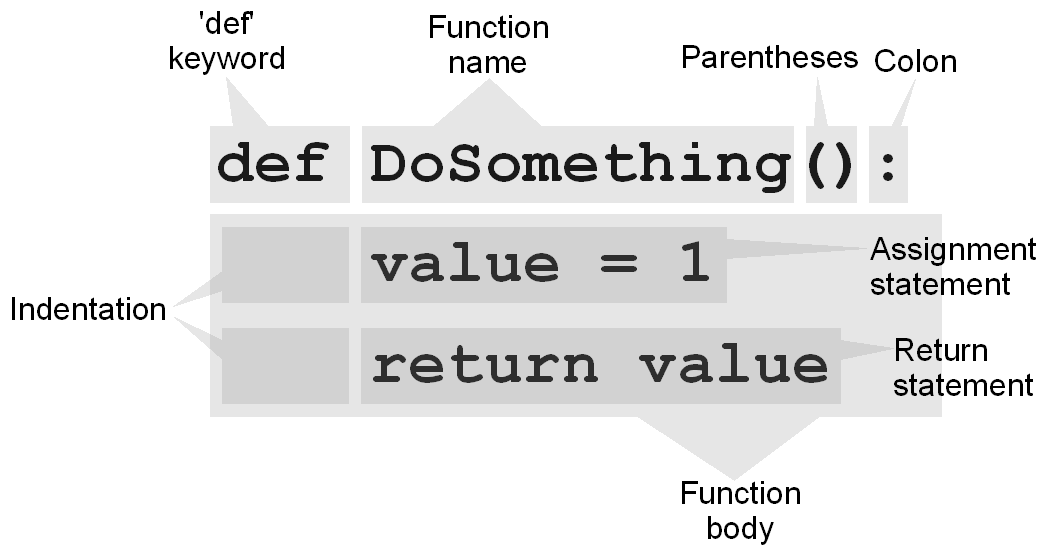
\includegraphics[width=0.7\textwidth]{images/function_def.png}
\end{center}
\end{frame}
\begin{frame}[label={sec:org1853957},fragile]{Skeleton of a function}
 \begin{block}{\texttt{def my\_fun(a, b, c="Two"):}}
\ldots{}. \texttt{if (a>2):}

\ldots{}\ldots{}.. \texttt{return 1}

\ldots{}. \texttt{else:}

\ldots{}\ldots{}..  \texttt{return (None, 3)}
\end{block}
\begin{itemize}
\item \alert{DEMO}
\item Arguments/Parameters \texttt{my\_fun(1,2,"Five")}
\item Return statements (none/one/many)
\item Default parameters \texttt{my\_fun(10, 12)}
\item Keyword parameters \texttt{my\_fun(4, b=2, c="One")}
\item Multiple returns through tuples
\item Arbitrary number of arguments also possible
\end{itemize}
\end{frame}
\begin{frame}[label={sec:org6cee0ee},fragile]{Practice}
 \begin{block}{Please attempt}
\texttt{07\_introduction\_to\_functions.ipynb}
\texttt{08\_some\_more\_functions.ipynb}
\end{block}
\end{frame}
\begin{frame}[label={sec:orgbf017b2},fragile]{Call by value/reference \#1?}
 What's the output of the following code block?
\footnotesize
\begin{minted}[]{python}
def side_effects(x):
    print("x =", x, " id =", id(x))
    x = 42.
    print("x =", x, " id =", id(x))

x = 3.14159
print("First call {0} with value {1}".format(id(x), x))
side_effects(x)
print("Second call {0} with value {1}".format(id(x), x))
\end{minted}
\begin{block}<2->{Output}
\footnotesize
\begin{verbatim}
First call 4381692976 with value 3.14159
x = 3.14159  id = 4381692976
x = 42.0  id = 4382805616
Second call 4381692976 with value 3.14159
\end{verbatim}
\end{block}
\end{frame}
\begin{frame}[label={sec:org6c4e37e},fragile]{Call by value/reference \#2?}
 What's the output of the following code block?
\footnotesize
\begin{minted}[]{python}
def side_effects(x):
    print("x =", x, " id =", id(x))
    x = x + ["aero", "civil"]
    print("x =", x, " id =", id(x))

x = ["cs","mechse","matse"]
print("First call {0} with value {1}".format(id(x), x))
side_effects(x)
print("Second call {0} with value {1}".format(id(x), x))
\end{minted}
\begin{block}<2->{Output}
\scriptsize
\begin{verbatim}
First call 4505434880 with value ['cs', 'mechse', 'matse']
x = ['cs', 'mechse', 'matse']  id = 4505434880
x = ['cs', 'mechse', 'matse', 'aero', 'civil']  id = 4503751040
Second call 4505434880 with value ['cs', 'mechse', 'matse']
\end{verbatim}
\end{block}
\end{frame}
\begin{frame}[label={sec:orgcbbd422},fragile]{Call by value/reference \#3?}
 What's the output of the following code block?
\footnotesize
\begin{minted}[]{python}
def side_effects(x):
    print("x =", x, " id =", id(x))
    x += ["aero", "civil"]
    print("x =", x, " id =", id(x))

x = ["cs","mechse","matse"]
print("First call {0} with value {1}".format(id(x), x))
side_effects(x)
print("Second call {0} with value {1}".format(id(x), x))
\end{minted}
\begin{block}<2->{Output}
\scriptsize
\begin{verbatim}
First call 4439456320 with value ['cs', 'mechse', 'matse']
x = ['cs', 'mechse', 'matse']  id = 4439456320
x = ['cs', 'mechse', 'matse', 'aero', 'civil']  id = 4439456320
Second call 4439456320 with value ['cs', 'mechse', 'matse', 'aero', 'civil']
\end{verbatim}
\end{block}
\end{frame}
\begin{frame}[label={sec:org4e79ec2}]{Call by value/reference}
\begin{alertblock}{Take-away}
Only mutable structures can be changed with in-place transformations!
\end{alertblock}
\end{frame}

\begin{frame}[label={sec:org3f8c054}]{Recursive functions}
\note{:B\_note:
\begin{itemize}
\item Ask them to do it
\end{itemize}}
\begin{itemize}
\item Recursion occurs in a lot of places (e.g. in trees---remember representation?)
\item Let's calculate factorial of a number
\end{itemize}
\begin{equation}
 n! = n \times (n-1) \times (n-2) \times \cdots \times 1
\end{equation}
\[ 7! = 5040 \]
\end{frame}

\begin{frame}[label={sec:org2eaf552},fragile]{Factorial done recursively}
 \begin{equation*}
 n! = n \times (n-1) \times (n-2) \times \cdots \times 1
\end{equation*}

\small
\begin{minted}[]{python}
def factorial(n):
    """ Calculates the factorial recursively """
    n = abs(int(n))
    if n == 0:
            return 1
    else:
            return n * factorial(n-1)

print(factorial(7))  #prints(5040)
\end{minted}
\end{frame}

\begin{frame}[label={sec:org38d7145},fragile]{Factorial done iteratively}
 \begin{equation*}
 n! = n \times (n-1) \times (n-2) \times \cdots \times 1
\end{equation*}

\small
\begin{minted}[]{python}
def factorial_iter(n):
    """ Calculates the factorial iteratively"""
    result = 1
    n = abs(int(n))
    for i in range(1, n+1):
        result *= i
    return result

print(factorial_iter(7))  #prints(5040)
\end{minted}
\end{frame}

\begin{frame}[label={sec:orgd3a6cd6}]{Which one is preferable?}
\begin{itemize}
\item Consider generating the Fibonacci sequence
\end{itemize}
\begin{equation*}
0, 1 , 1 , 2 , 3 , 5 , 8 , 13 , 21 , \cdots
\end{equation*}
\begin{itemize}
\item Recursive formula is
\end{itemize}
\begin{equation}
F_{N} = F_{N-1} + F_{N-2}
\end{equation}
\begin{itemize}
\item \alert{Fibonacci.ipynb}
\end{itemize}
\end{frame}
\begin{frame}[label={sec:org920e904},fragile]{Towers of Hanoi}
 \begin{alertblock}{Prefer iteration when possible}
But not always! Let's solve Towers of Hanoi\ldots{}
\end{alertblock}
\begin{block}{Activity}
Write a \texttt{Python} script that solves the game ``Towers of Hanoi''\footnote{\href{https://commons.wikimedia.org/wiki/File:Tower\_of\_Hanoi.jpeg}{Tower of Hanoi, Wikimedia Commons}}. Hint:
Recursion is key.
\end{block}
\footnotesize
\begin{figure}[htbp]
\centering
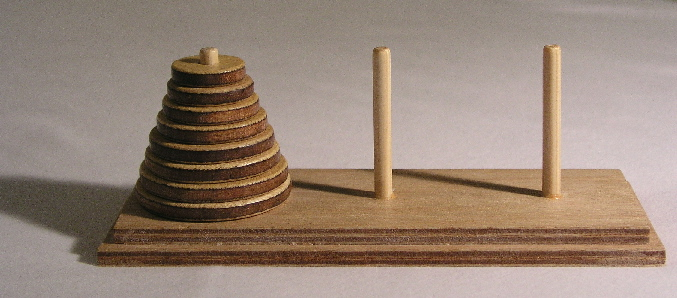
\includegraphics[width=0.7\textwidth]{images/hanoi.jpeg}
\caption{Tower of Hanoi}
\end{figure}
\end{frame}
\begin{frame}[label={sec:orgcb7f9c3}]{Solution strategy \footnote{\href{https://www.cs.sfu.ca/\~tamaras/recursion/Rules\_Towers\_Hanoi.html}{Computing Science - Simon Fraser University}}}
\begin{columns}
\begin{column}{0.5\columnwidth}
\begin{itemize}
\item The fourth step besides is key!
\item A \(n\)-disk game should have the same step
\item Recursive solution naturally pops out!
\item Iterative solution is difficult\ldots{}
\end{itemize}
\end{column}
\begin{column}{0.4\columnwidth}
\begin{figure}[htbp]
\centering
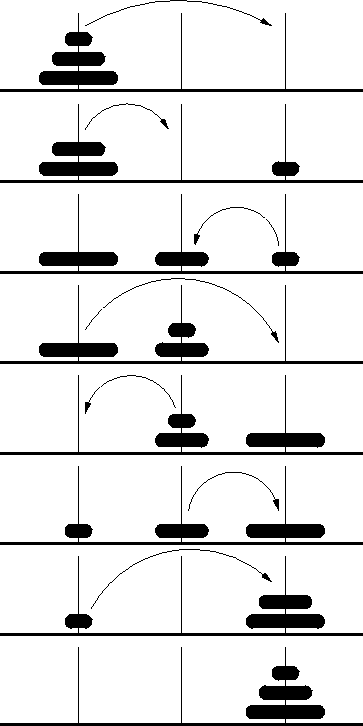
\includegraphics[width=0.7\textwidth]{images/toh_sol.png}
\caption{Three disk solution}
\end{figure}
\end{column}
\end{columns}
\end{frame}

\begin{frame}[label={sec:org56855ca},fragile]{Towers of Hanoi}
 \footnotesize
\begin{minted}[]{python}
def hanoi(n, source, helper, target):
    if n > 0:
        # move tower of size n - 1 to helper:
        hanoi(n - 1, source, target, helper)
        # move disk from source peg to target peg
        if source:
            target.append(source.pop())
        # move tower of size n-1 from helper to target
        hanoi(n - 1, helper, source, target)

N_DISKS = 6
source = list(range(N_DISKS, 0, -1))
target = []; helper = [];
hanoi(len(source),source,helper,target)
\end{minted}
\note{:B\_note:
\begin{itemize}
\item Interestingly using tree representation, you can naturally evolve this program!
\end{itemize}}
\end{frame}

\begin{frame}[label={sec:org1a24bd1},fragile]{Basic I/O}
 \begin{itemize}
\item We frequently (but not consciously) manipulate files everyday.
\item Here's how you do it in \texttt{Python}
\footnotesize
\begin{minted}[]{python}
# 'r' for read mode
fobj = open("show_me_to_the_class.txt", 'r')
for line in fobj:
    print(line.rstrip())
fobj.close()
\end{minted}

\item ---OUTPUT---
\begin{verbatim}
I am a file whose contents the class needs to see.
\end{verbatim}
\end{itemize}


\begin{itemize}
\item Finally remember that \texttt{print} can also write to files
\item \texttt{shell} example of file manipulation using \texttt{>>, >}
\end{itemize}
\end{frame}
\begin{frame}[label={sec:orge46b121},fragile]{Basic I/O continued}
 \begin{itemize}
\item A safer way to do I/O is
\footnotesize
\begin{minted}[]{python}
# 'r' for read mode
with open("show_me_to_the_class.txt", 'r') as fobj:
    for line in fobj:
        print(line.rstrip())
\end{minted}

\item ---OUTPUT---
\begin{verbatim}
I am a file whose contents the class needs to see.
\end{verbatim}
\end{itemize}


\begin{itemize}
\item The same mechanism can be used to write to a file
\footnotesize
\begin{minted}[]{python}
# 'w' for write mode, 'a' for append mode
# 'w' wipes a file clean before it writes
# This creates a file if it doesn't exist
with open("show_me_to_the_class_two.txt", 'w') as fobj:
    fobj.write("Are prequels better? \n Obviously! \n")
\end{minted}
\end{itemize}
\end{frame}

\begin{frame}[label={sec:org58fb9c4},fragile]{Basic I/O continued}
 \begin{itemize}
\item For smaller files, you can read them completely into a list
\footnotesize
\begin{minted}[]{python}
fullfl = open("show_me_to_the_class.txt", 'r').readlines()
print(fullfl)
\end{minted}

\item ---OUTPUT---
\begin{verbatim}
['I am a file whose contents the class needs to see.']
\end{verbatim}
\end{itemize}


\begin{itemize}
\item \texttt{read()} instead of \texttt{readlines()} does the same thing, but with subtle differences
\end{itemize}
\end{frame}

\begin{frame}[label={sec:org2e5c1c4},fragile]{Basic I/O continued}
 \begin{itemize}
\item Later on we will see how to store matrices and arrays using the \texttt{loadtxt}
and \texttt{savetxt} methods from \texttt{numpy}
\item Other packages also have many I/O options---for example \texttt{Pandas} has many
\texttt{csv} manipulations
\item Serialization (load/store as bytestrings) packages like \texttt{pickle, shelve}
also exist
\item In short, quite a lot of options!
\end{itemize}
\end{frame}

\begin{frame}[label={sec:org78aa75f},fragile]{Counting Words}
 \begin{block}{Activity}
Write a \texttt{Python} script that reads in a file and print out the number of
words

Download Goldilocks: \url{http://www.textfiles.com/stories/gold3ber.txt}
\end{block}
\end{frame}

\begin{frame}[label={sec:orgd3879c5},fragile]{Classes : Object oriented programming}
 \begin{itemize}
\item A logical entity that groups variables and functions together!
\footnotesize
\begin{minted}[]{python}
class Point:
    """ A point class with (x,y) coords and manipulations
    """
    def __init__(self, x, y):
        """ Create new point at x,y"""
        self.x = x; self.y = y
    def translate(self, t_x, t_y):
        """ Translate by some distance"""
        self.x += t_x; self.y += t_y
    # Other members follow
p = Point(1.0, 0.0)
\end{minted}
\end{itemize}


\begin{itemize}
\item The \texttt{class} has \alert{attributes} (or variables) and \alert{methods} (functions that
act on the attributes)
\item \texttt{init} is a special method
\end{itemize}
\end{frame}
\begin{frame}[label={sec:org23b9759},fragile]{Classes : Object oriented programming}
 We have come a full circle! All variables (ints, floats, sequences) are
classes in \texttt{Python}!!!
\end{frame}
\begin{frame}[label={sec:org9a4015c},fragile]{Modules}
 \note{:B\_note:
\begin{itemize}
\item Show obscurity on what function is running
\item from numpy import $\backslash$*, from math import $\backslash$*, sin(3)? Which is called?
\item Answer: The one corresponding to the last import. That means
\item from math import $\backslash$*, from numpy import $\backslash$*, sin(3)? gives different answers
\end{itemize}}

\begin{itemize}
\item Modular design \(\rightarrow\) modules\ldots{}
\item \texttt{import math} imports a module and its contents to the current program
\item Selective import using \texttt{from} : \texttt{from math import sin, cos}
\item Importing all functions from a module : \texttt{from math import *}
\item Bad idea! \alert{DEMO}
\item You can also design your own modules\ldots{} But it soon becomes painful.
\item \texttt{Python's} answer : packages!
\end{itemize}
\end{frame}

\begin{frame}[label={sec:orgfba9df3},fragile]{Packages}
 \begin{itemize}
\item Packages: make publicly available modules that other people have written
\item You installed packages from \texttt{pip} at the start of the semester!
\item Packages of our interest : \texttt{numpy}, \texttt{scipy}, \texttt{matplotlib}\ldots{}
\end{itemize}
\end{frame}
\begin{frame}[label={sec:orgcefcbb6},fragile]{Why do we need numpy/ scipy/ matplotlib?}
 \begin{itemize}
\item \alert{Jupyter demo} for matrix computation
\item \alert{numpy} : Basic scientific computing powerhorse
\item \alert{scipy} : More targeted, \emph{advanced} algorithms
\item \alert{matplotlib} : Basic (?!) plotting library
\item The scientific computing eco-system in \texttt{Python} \textsuperscript{\cref{org6dcf9e0}}
\end{itemize}
\begin{center}
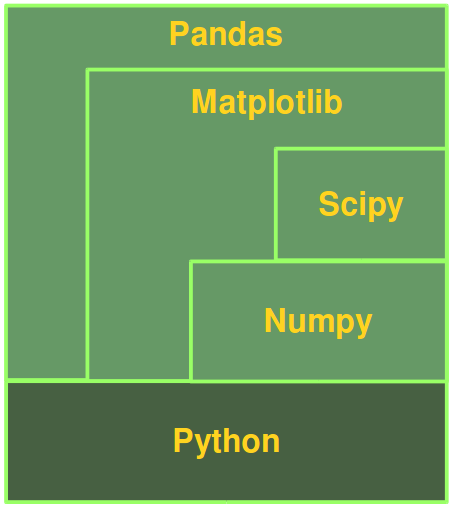
\includegraphics[width=0.4\textwidth]{images/python_numerics.png}
\end{center}
\end{frame}
\note{Examples
\begin{itemize}
\item Count number of words in a text files
\item Play a game of tower of Hanoi
\item Os module for path and file manipulations
\item \url{http://hplgit.github.io/INF5620/doc/pub/H14/vib/sphinx/.\_main\_vib001.html}
\end{itemize}}

\note{Packages to be shown
\begin{itemize}
\item Scipy x 2
\item Matplotlib x 1
\item Sympy x 1
\item Pandas x 1
\item Os module for path and file manipulations x 1
\item Seaborn x 1
\item \url{http://hplgit.github.io/INF5620/doc/pub/H14/vib/sphinx/.\_main\_vib001.html}
\end{itemize}}
\end{document}
